%\title{LaTeX Portrait Poster Template}
%%%%%%%%%%%%%%%%%%%%%%%%%%%%%%%%%%%%%%%%%
% a0poster Portrait Poster
% LaTeX Template
% Version 1.0 (22/06/13)
%
% The a0poster class was created by:
% Gerlinde Kettl and Matthias Weiser (tex@kettl.de)
% 
% This template has been downloaded from:
% http://www.LaTeXTemplates.com
%
% License:
% CC BY-NC-SA 3.0 (http://creativecommons.org/licenses/by-nc-sa/3.0/)
%
%%%%%%%%%%%%%%%%%%%%%%%%%%%%%%%%%%%%%%%%%

%----------------------------------------------------------------------------------------
% PACKAGES AND OTHER DOCUMENT CONFIGURATIONS
%----------------------------------------------------------------------------------------

\documentclass[a0,landscape]{a0poster}
\usepackage[utf8]{inputenc}
\usepackage{algorithm}
\usepackage{algorithmicx}
\usepackage{algpseudocode}
\usepackage{multicol} % This is so we can have multiple columns of text side-by-side
\usepackage{subfigure}
\columnsep=100pt % This is the amount of white space between the columns in the poster
\columnseprule=3pt % This is the thickness of the black line between the columns in the poster

\usepackage[svgnames]{xcolor} % Specify colors by their 'svgnames', for a full list of all colors available see here: http://www.latextemplates.com/svgnames-colors

%\usepackage{empheq}
\usepackage[most]{tcolorbox}

\tcbset{colback=yellow!10!white, colframe=red!50!black, 
        highlight math style= {enhanced, %<-- needed for the ’remember’ options
            colframe=red,colback=red!10!white,boxsep=0pt}
        }

\definecolor{opticlimb}{rgb}{0,0.65,0.65}
\definecolor{blue}{RGB}{0,0,255}
\usepackage{tcolorbox}

% \usepackage[bitstream-charter]{mathdesign}
\usepackage[authoryear,round]{natbib}
\usepackage{bbm}
\usepackage{enumitem} 
\usepackage{xargs} 
\usepackage{amssymb,amsthm,bm}
%\usepackage{mathtools}
%\usepackage{xargs}
%\usepackage{stmaryrd} 

\bibliographystyle{plainnat}
\usepackage{graphicx} % Required for including images
\graphicspath{{figures/}} % Location of the graphics files
\usepackage{booktabs} % Top and bottom rules for table
%\usepackage[font=small,labelfont=bf]{caption} % Required for specifying captions to tables and figures
%\usepackage{amsfonts, amsmath, amsthm, amssymb,bm} % For math fonts, symbols and environments
\usepackage{wrapfig} % Allows wrapping text around tables and figures

\usepackage{cmbright}
\usepackage{avant}
%\usepackage{tikz}
%\usepackage[T1]{fontenc}
%\usepackage[utf8]{inputenc}
%\usepackage[font=small,labelfont=bf,tableposition=top]{caption}

\renewcommand{\familydefault}{\sfdefault}
\theoremstyle{definition}
\newtheorem{defn}{Definition} % definition numbers are dependent on theorem numbers
\newtheorem*{exmp}{Example} % same for example numbers
\newtheorem{assumption}{H\!\!}

\usepackage{mdframed}
%\theoremstyle{definition}
%\newtheorem{defn}{Definition} % definition numbers are dependent on theorem numbers
%\newtheorem*{exmp}{Example} % same for example numbers
%\usepackage{lipsum}%
%  {
%      \theoremstyle{plain}
%      \newtheorem{assumption}{M}
%      \newtheorem{lemma}{Lemma}
%      \newtheorem{remark}{Remark}
%      \newtheorem{prop}{Proposition}
%      \newtheorem{assumption_saem}{ISAEM}
%      \newtheorem{assumption_rm}{SA}
%      \newtheorem{assumption_iem}{IEM}
%      \newtheorem{assumption_imcem}{IMCEM}
%      \newtheorem{assumption_expo}{E}
%  }
\newmdtheoremenv{theo}{Theorem}
\newmdtheoremenv{coro}{Corollary}
\newmdtheoremenv{lem}{Lemma}

\usepackage{shortcuts_OPT}

\begin{document}

{~\hspace{6cm}\begin{tikzpicture}[remember picture, overlay]
     \node [anchor=north east, inner sep=3cm, yshift=-5.5cm]  at (current page.north east)
     {
\includegraphics[height=6cm]{images/logo_baidu.jpeg}
       
\includegraphics[height=5cm]{images/logo_cuhk.png}~~
     
\includegraphics[height=5cm]{images/logo_x.jpg}};
  \end{tikzpicture}}
  
  \begin{tikzpicture}[remember picture, overlay]
     \node [inner sep=3cm, yshift=2cm]  at (current page.south)
     {\large The 33rd International Conference on Algorithmic Learning Theory};
  \end{tikzpicture}
%----------------------------------------------------------------------------------------
% POSTER HEADER 
%----------------------------------------------------------------------------------------

% The header is divided into two boxes:
% The first is 75% wide and houses the title, subtitle, names, university/organization and contact information
% The second is 25% wide and houses a logo for your university/organization or a photo of you
% The widths of these boxes can be easily edited to accommodate your content as you see fit

\begin{minipage}[b]{0.9\linewidth}
\veryHuge \color{Navy} \textbf{Minimization by Incremental Stochastic Surrogate Optimization for Large Scale Nonconvex Problems
}\\[1cm] \color{Black} %\color{Black}\textbf{COLT 2019} \color{Black}\\[1cm] % Title
%\Huge\textit{Identification de système dynamique}\\[2cm] % Subtitle
\huge \textbf{Belhal Karimi$^{1}$, Hoi-To Wai$^{2}$, Eric Moulines$^{3}$ and Ping Li$^{1}$}\\[0.5cm] % Author(s)
\huge Baidu Research$^1$, Chinese University~of Hong Kong$^2$, Ecole Polytechnique$^3$ \\[0.4cm] % University/organization
\large \texttt{belhalkarimi@baidu.com, htwai@se.cuhk.edu.hk, eric.moulines@polytechnique.edu, liping11@baidu.com@gmail.com}
\end{minipage}
%


\vspace{1cm} % A bit of extra whitespace between the header and poster content

%----------------------------------------------------------------------------------------

\begin{multicols}{3} % This is how many columns your poster will be broken into, a portrait poster is generally split into 2 columns

%----------------------------------------------------------------------------------------
% ABSTRACT
%----------------------------------------------------------------------------------------




%----------------------------------------------------------------------------------------
% INTRODUCTION
%----------------------------------------------------------------------------------------

%\color{SaddleBrown} % SaddleBrown color for the introduction
%\color{Navy} % Navy color
%\color{opticlimb}
%\color{Navy} % Navy color for the abstract
\color{DarkSlateGray}


\begin{tcolorbox}[colback=white!5!white,colframe=green!75!black,fonttitle=\sffamily\bfseries\large,title=Large Scale Optimization]
\begin{itemize}
\item \textbf{Objective:} \emph{Constrained} minimization problem of a finite sum of  functions:
\beq \label{eq:opt}
\min_{ \param \in \Param }~ {\cal L} ( \param ) \eqdef \frac{1}{n} \sum_{i=1}^n {\cal L}_i( \param) \eqsp,
\eeq
where ${\cal L} _i: \rset^p \to \rset$ is bounded from below and is (possibly) nonconvex and include a nonsmooth penalty.
\item The gap $\widehat{e}(\param ; \{ \op_i \}_{i=1}^n )$ is L-smooth.
Denote by $\pscal{\cdot}{\cdot}$ the scalar product, the stationary point condition is:
\begin{defn} (Asymptotic Stationary Point Condition)\\
A sequence $(\theta^k)_{k\geq0}$ satisfies the asymptotic stationary point condition if
\begin{equation}\label{aspc}
f'( \param, {\bm d} ) \eqdef \lim_{ t \rightarrow 0^+ } \frac{ f ( \param + t {\bm d} ) - f( \param ) }{ t }  \geq 0.
\end{equation}
\end{defn}
\end{itemize}
\vspace{.1cm}
\end{tcolorbox}

\begin{tcolorbox}[colback=white!5!white,colframe=blue!75!black,fonttitle=\sffamily\bfseries\large,title=Majorization-Minimization Scheme]
\begin{itemize}
%\item dd
%
%\begin{figure}[H]
%\centering
%        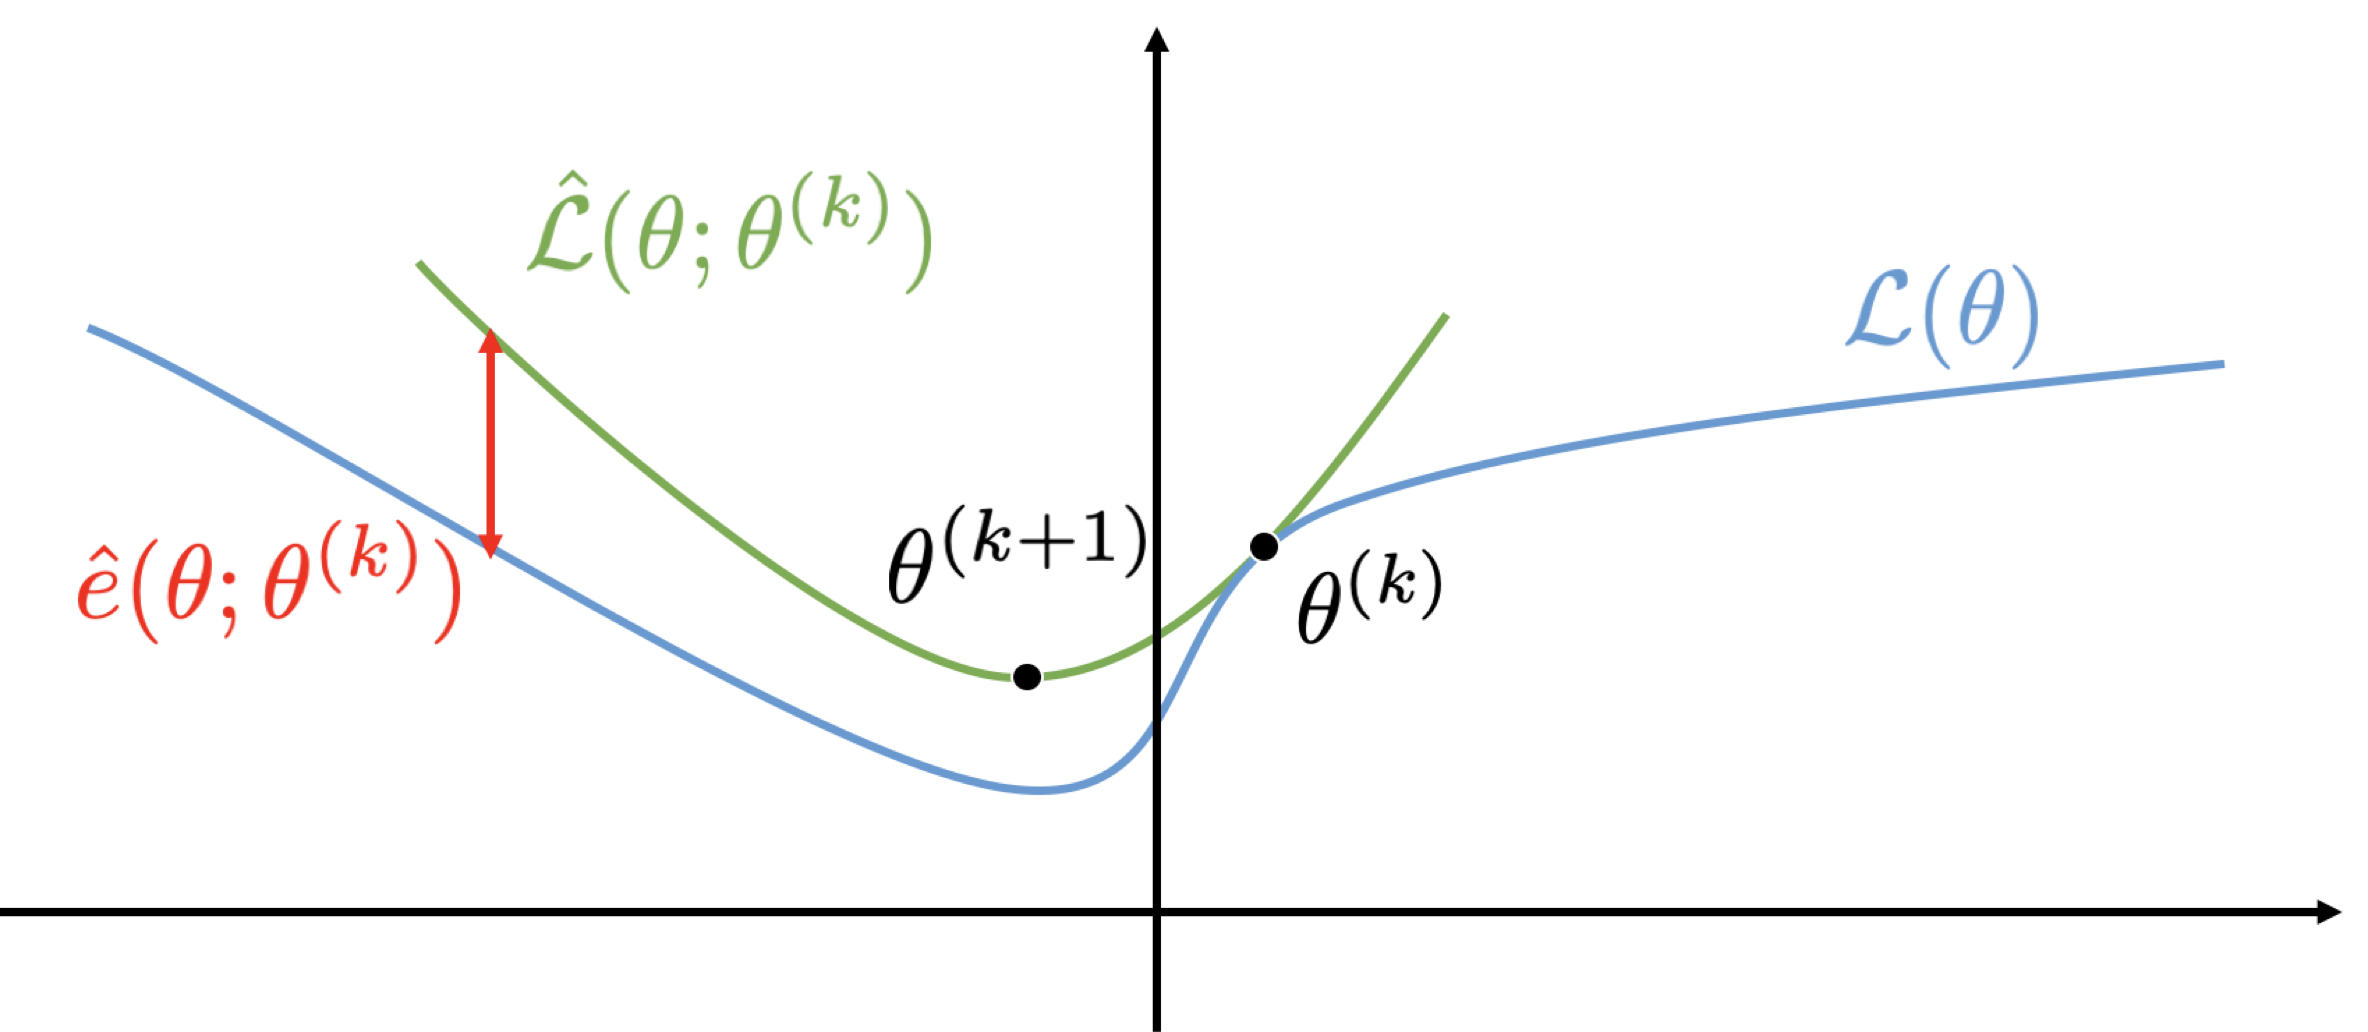
\includegraphics[width=0.5\textwidth]{fig/mmscheme}
%\end{figure} 
%

\item The MISO method~\citep{mairal2015miso}
\begin{figure}[H]
\centering
        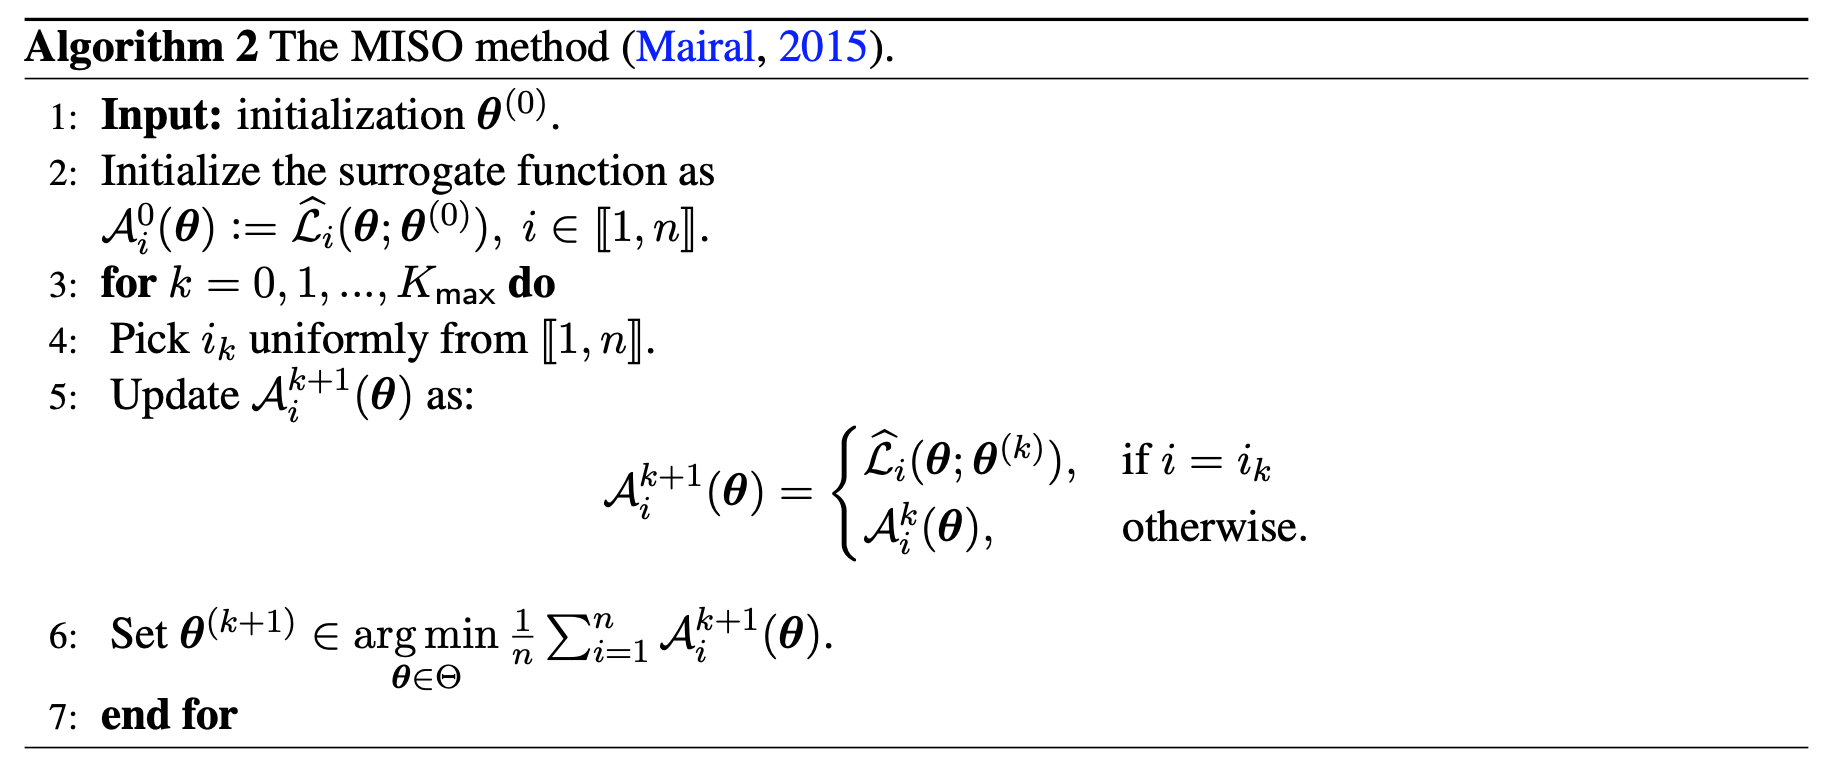
\includegraphics[width=1.0\textwidth]{fig/misoalgofull}
\end{figure} 
\end{itemize}
\end{tcolorbox}

\begin{tcolorbox}[colback=white!5!white,colframe=blue!75!black,fonttitle=\sffamily\bfseries\large,title=An Inctractability for Latent Data Models]
\begin{itemize}[label=\textbullet, font=\LARGE \color{blue}]
\item Case when the surrogate functions computed in Algorithm \ref{alg:miso} \textbf{are not tractable}.
\item Assume that the surrogate can be expressed as an integral over a set of latent variables $z = (z_i \in \Zset, i \in [n]) \in \Zset[]$.
\begin{tcolorbox}[colback=red!5!white,colframe=red!75!black]
\begin{equation}\label{eq:integralsurrogate}
\sur{i}{\param}{\op} \eqdef \int_{\Zset}{\rsur{i}{\param}{\op}{z_i}  p_i(z_i ; \op)\mu_i(dz_i)}\quad \forall~(\param,\op) \in \Param \times \Param \eqsp.
\end{equation}
\end{tcolorbox}  

\item Our scheme is based on the computation, at each iteration, of stochastic auxiliary functions for a mini-batch of components. For $i \in [n]$, the auxiliary function, noted $\ssur{i}{\param}{\op}{ \{ z_m \}_{m=1}^{M}}$ is a Monte Carlo approximation of the surrogate function $\sur{i}{\param}{\op}$ defined by \eqref{eq:integralsurrogate} such that:
\begin{tcolorbox}[colback=green!5!white,colframe=green!75!black]
\beq \label{eq:ssur}  
\ssur{i}{\param}{\op}{ \{ z_m \}_{m=1}^{M}} \eqdef \frac{1}{M} \sum_{m=1}^{M} \rsur{i}{\param}{\op}{z_m}\eqsp,
\eeq
\end{tcolorbox}
where $\{z_i^{m}\}_{m=0}^{M-1}$ is a Monte Carlo batch.
\end{itemize}

\vspace{.1cm}
\end{tcolorbox}


\begin{tcolorbox}[colback=white!5!white,colframe=blue!75!black,fonttitle=\sffamily\bfseries\large,title=MISSO Method]
\begin{figure}[H]
\centering
        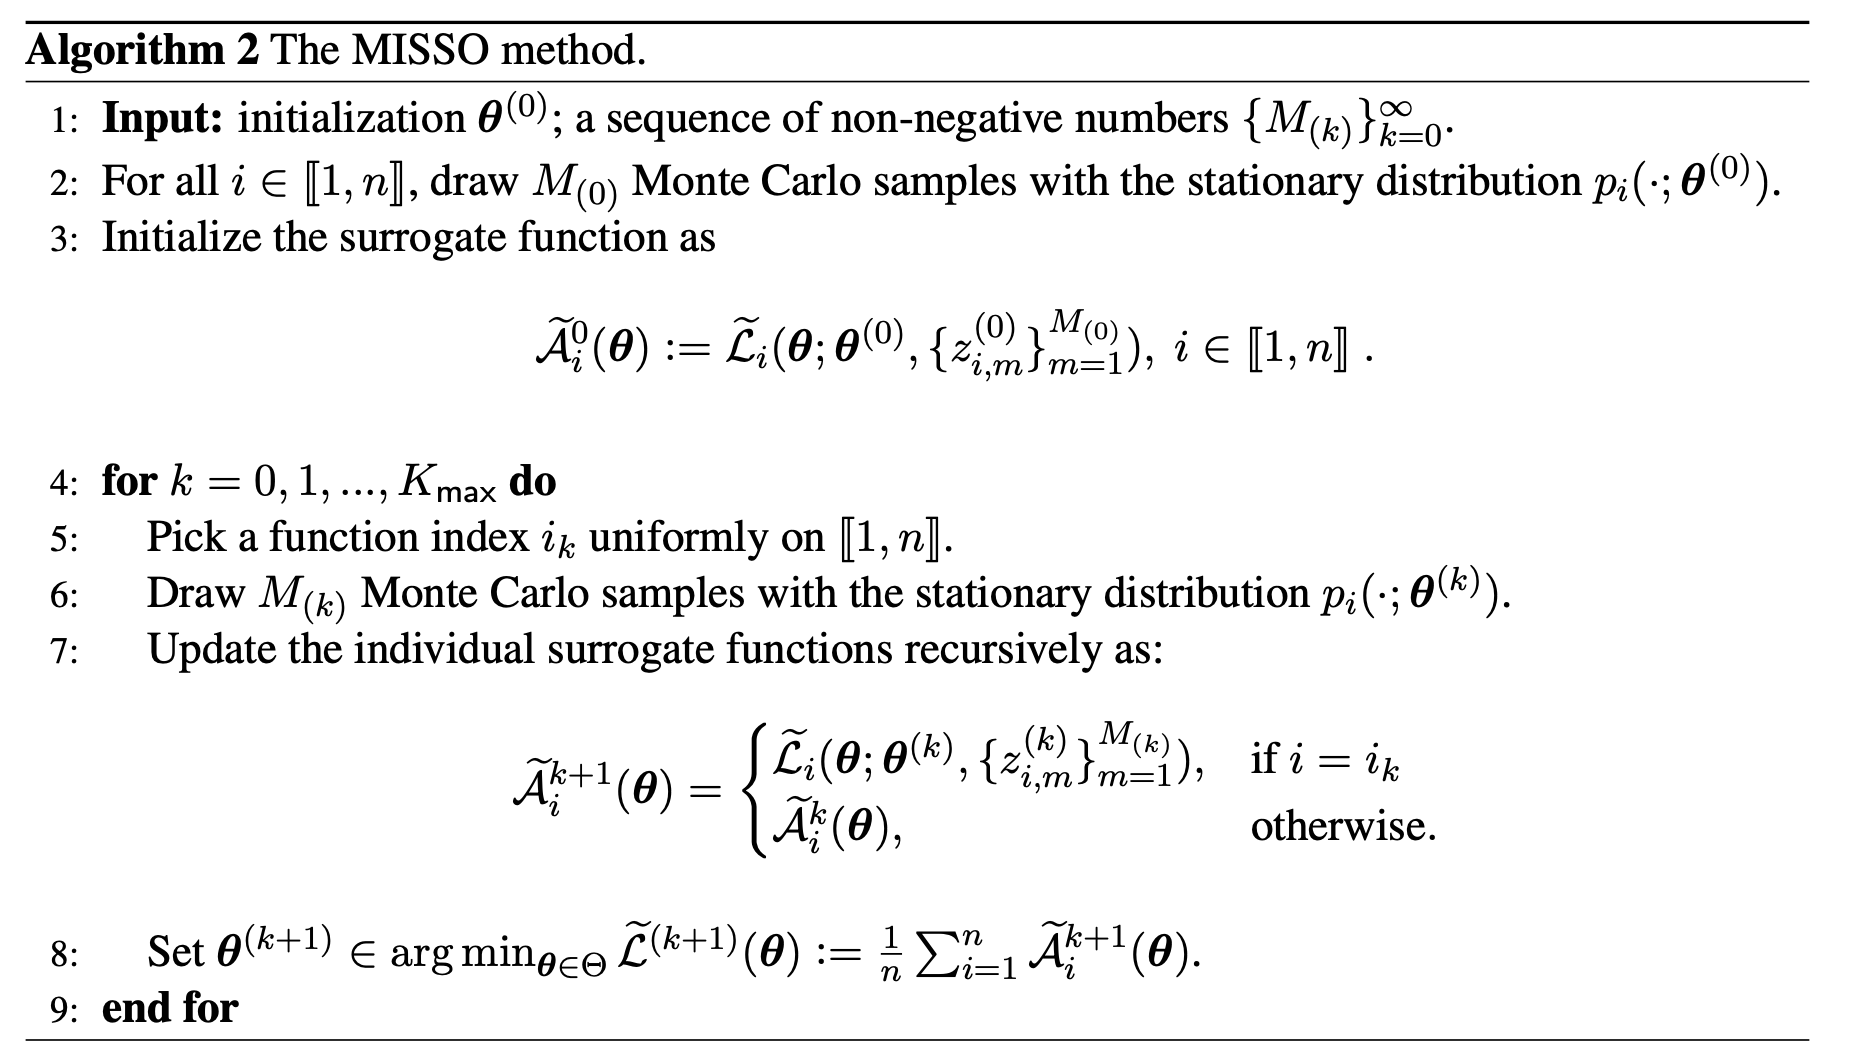
\includegraphics[width=1.\textwidth]{fig/missoalgo}
\end{figure}
\end{tcolorbox}


\begin{tcolorbox}[colback=white!5!white,colframe=red!75!black,fonttitle=\sffamily\bfseries\large,title=Global Convergence Analysis]
\textbf{Assumptions}: we need a few regularity conditions in this case,
\begin{assumption} \label{ass:sur} For all $i \in [n]$ and $\op \in \Param$, $\sur{i}{\param}{\op}$ is convex \wrt $\param$, and it holds
$\sur{i}{\param}{\op} \geq {\cal L}_i( \param ),~\forall~\param \in \Param$ where the equality holds when $\param = \op$.
\end{assumption}
\begin{assumption} \label{ass:diff}
For any $\op_i \in \Param$, $i \in [n]$ and some $\epsilon > 0$, the difference function $\widehat{e}(\param ; \{ \op_i \}_{i=1}^n ) \eqdef \frac{1}{n} \sum_{i=1}^n \sur{i}{\param}{\op_i } - {\cal L}( \param)$ is defined for all $\param \in \Param_\epsilon$ and differentiable for all $\param \in \Param$, where $\Param_\epsilon = \{ \param \in \rset^d, \inf_{\param' \in \Param} \| \param - \param' \| < \epsilon \}$ is an $\epsilon$-neighborhood set of $\Param$. Moreover, for some constant $L$, the gradient satisfies $\| \grd \widehat{e}(\param; \{ \op_i \}_{i=1}^n)  \|^2 \leq 2 L\!~ \widehat{e}(\param; \{ \op_i \}_{i=1}^n) ,~\forall~\param \in \Param$.
\end{assumption}
\begin{assumption} \label{ass:lips}
For all $i \in [n]$, $\op \in \Param$, $z_i \in \Zset$, $\rsur{i}{\cdot}{\op}{z_i}$ is convex on $\Param$ and is lower bounded.
\end{assumption}\vspace{-0.1in}

\begin{assumption}\label{controlapprox}
For the samples $\{z_{i,m}\}_{m=1}^{M}$, there exist finite constants $C_{\sf r}$ and $C_{\sf gr}$ such that for all $i \in [n]$,
\beq\notag
C_{\sf r} \eqdef \sup \limits_{\op \in \Param} \sup \limits_{M >0} \frac{1}{\sqrt{M}} \EE_{\op}\left[ \sup \limits_{\param \in \Param} \left| \sum_{m=1}^{M}{ \left\{ r_i (\param ; \op, z_{i,m})  - \sur{i}{\param}{\op} \right\} } \right| \right]
\eeq
\beq\notag
C_{\sf gr} \eqdef \sup \limits_{\op \in \Param} \sup \limits_{M >0} \sqrt{M} \EE_{\op}\left[ \sup \limits_{\param \in \Param} \left| \frac{1}{{M}} \sum_{m=1}^{M}{ \frac{
 \widehat{\cal L}_i'( \param , \param - \op; \op ) - r_i' (\param, \param - \op ; \op,  z_{i,m} ) }{\| \op - \param\|} }\right|^2 \right]
\eeq
where we denoted by $\mathbb{E}_{\op} [\cdot]$ the expectation \wrt a Markov chain $\{z_{i,m}\}_{m=1}^{M}$ with  initial distribution $\xi_{i} (\cdot; \op)$, transition kernel $\Pi_{i,\op}$, and stationary distribution $p_{i}(\cdot; \op)$.
\end{assumption}
\begin{figure}[H]
\centering
        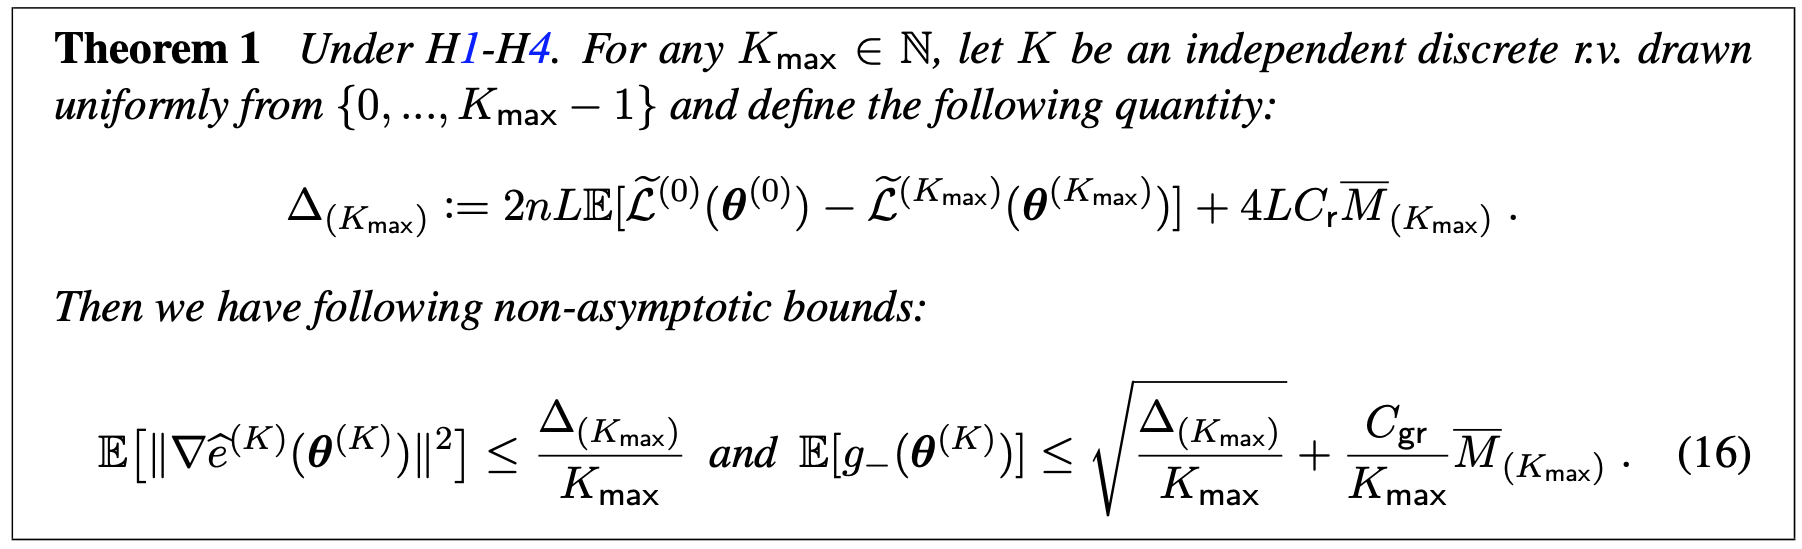
\includegraphics[width=1.0\textwidth]{fig/theorem1}
\end{figure} 

\end{tcolorbox}


\begin{tcolorbox}[colback=white!5!white,colframe=red!75!black,fonttitle=\sffamily\bfseries\large,title=Numerical Experiments]
\begin{itemize}
\item Logistic Regression \textbf{with missing values} on Traumabase (severe hemorrhage):
\beq\notag
p_i(y_i|z_i) =  S({\bm \delta}^\top \bar{z}_i)^{y_i} \left(1 - S({\bm \delta}^\top \bar{z}_i)\right)^{1-y_i}\eqsp,
\eeq
\item $16$ quantitative measurements, like BMI, age, blood pressure, heart rate at different stages after the accident on $6384$ patients
\item \textbf{MISSO is an incremental MCEM in this case}
\begin{figure}[H]
\centering
    \mbox{
        \includegraphics[width=0.5\textwidth]{fig/logisticdelta.eps}
        \includegraphics[width=0.5\textwidth]{fig/logisticbeta.eps}
    }
\end{figure} 

\item Bayesian variants of LeNet-5 and ResNet-18 on MNIST and CIFAR10:
\item Variational inference and the ELBO loss to fit Bayesian Neural Networks on different datasets.
\item \textbf{MISSO is an incremental VI in this case}
\begin{figure}[H]
\centering
    \mbox{
        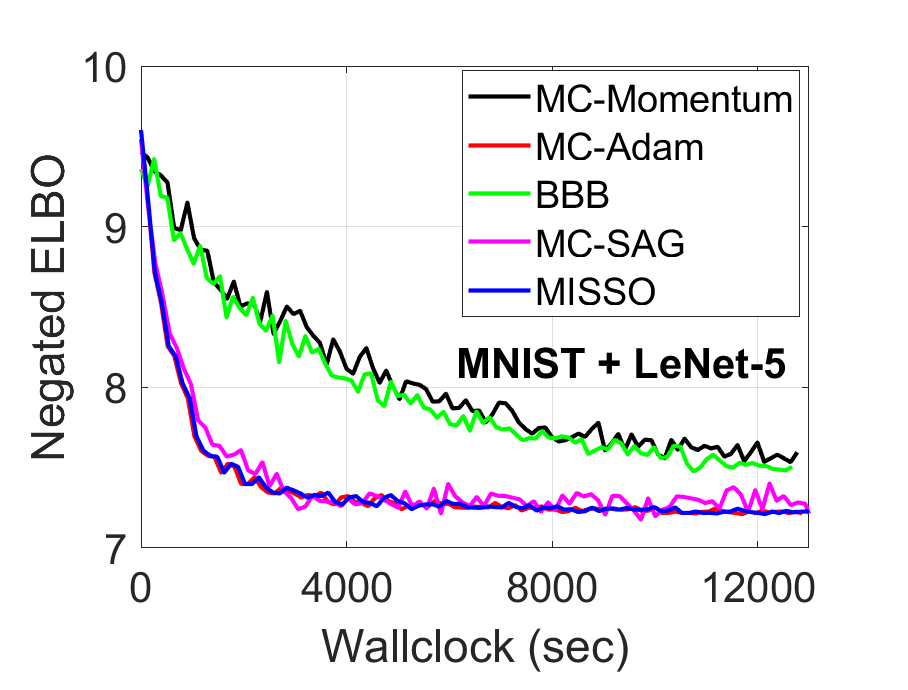
\includegraphics[width=0.5\textwidth]{fig/mnist.eps}
        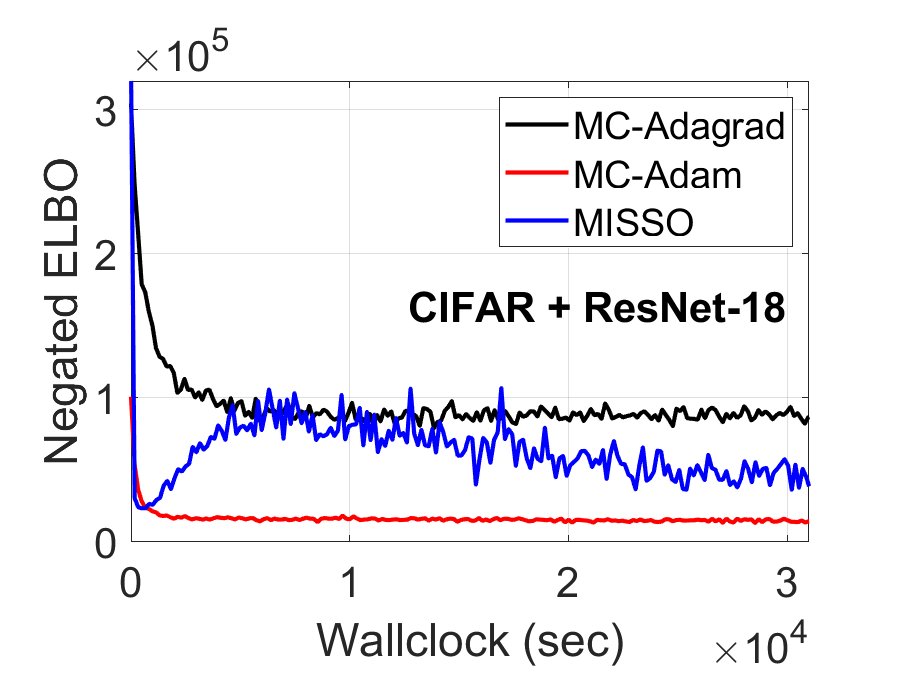
\includegraphics[width=0.5\textwidth]{fig/cifar.eps}
    }
\label{fig:gmmplots}
\end{figure} 
\end{itemize}
\end{tcolorbox}

\begin{tcolorbox}[colback=white!5!white,colframe=blue!75!black,fonttitle=\sffamily\bfseries\large,title=Conclusion]
\begin{itemize}
\item {\color{blue} Theorem 1 \& 2} show the non-asymptotic convergence rate of biased SA scheme with smooth (possibly non-convex) Lyapunov function. 
\item With appropriate step size, in \emph{n} iterations the SA scheme finds 
$\EE[ \| h( \prm_N ) \|^2 ] = {\cal O}( c_0 + \log n / \sqrt{n} )$, where $c_0$ is the bias and $h(\cdot)$ is the mean field.
\item Applications to online EM and online policy gradient.
\end{itemize}
\end{tcolorbox}
\vspace{-1.3cm}
\small
%\nocite{*} % Print all references regardless of whether they were cited in the poster or not
\bibliography{ref.bib}

%----------------------------------------------------------------------------------------
% ACKNOWLEDGEMENTS
%----------------------------------------------------------------------------------------

%\section*{Acknowledgements}

%\includegraphics[width=15cm]{opticlimb.png}\\


%----------------------------------------------------------------------------------------

\end{multicols}
\begin{center}
%
\includegraphics[width=10cm]{logo_x.jpg}
%
\includegraphics[width=10cm]{logo_inria.png}
%\includegraphics[width=15cm]{opticlimb.png}\\
\end{center}
\end{document}